% Lecture 7
\subsection{CNN}
\label{sub:cnn}
    \textbf{Integral operator}: Transform expressible with kernel $H$ s.t. for any function $f$ (for which $Tf$ exists): $(Tf)(u)=\int^{t_2}_{t_1}H(u,t)f(t)dt$ (eg: Fourier transform)
    
    \textbf{Convolution}: Given two functions $f,h$, their convolution is defined as:
    
    \tab $(f*h)(u)\coloneqq\int_{-\infty}^{\infty}h(u-t)f(t)dt=\int_{-\infty}^{\infty}f(u-t)h(t)dt $
    
    Integral operator with kernel $H(u,t)=h(u-t)$, shift-invariant as $H(u-s,t-s)=h(u-t)=H(u,t)\>(\forall s)$, commutative, typical use: $f$ signal, $h$ fast decaying kernel function.
    
    To generalize to higher dimensions: Replace vectors by matrices (for discrete case), tensors for 3D and higher.
    
    \tab $(F*G)\lbrack i,j \rbrack = \sum^\infty_{k=-\infty}\sum^\infty_{l=-\infty}F\lbrack i-k, j-l \rbrack \cdot G\lbrack k,l \rbrack$
    
    \textbf{Linear transform} $T$ is linear, if for all functions $f,g$ and scalars $\alpha,\beta$: 
    
    \tab$T(\alpha f+\beta g)=\alpha Tf+\beta Tg$
    
    \textbf{Translation invariant transform} $T$ is translation/shift invariant, if for any $f$ and scalar $\tau$,
    \tab$f_\tau(t)\coloneqq f(t+\tau),\>(Tf_\tau)=(Tf)(t+\tau)$
    
    Any linear, translation-invariant transformation $T$ can be written as a convolution with suitable $h$.
    
    \textbf{Discrete Cross-Correlation Vs Convolution}: Let $f,h:\mathbb{Z}\xrightarrow{}\R$, then:
    
    \tab$(h\star f)\lbrack u \rbrack\coloneqq\sum\limits^\infty_{t=-\infty}h\lbrack t \rbrack f \lbrack u+t \rbrack$. aka ``sliding inner product'', $u+t$ vs $u-t$
    
    Cross-correlation and convolution are closely related:
    
    \tab$(h\star f)\lbrack u \rbrack=\sum\limits^\infty_{t=-\infty}h\lbrack t \rbrack f \lbrack u+t \rbrack=\sum\limits^\infty_{t=-\infty}h\lbrack -t \rbrack f \lbrack u-t \rbrack$\\
    \tab$\phantom{(h\star f)\lbrack u \rbrack}=(\bar{h}*f)\lbrack u \rbrack=(f*\bar{h})\lbrack u \rbrack,\>\text{where } \bar{h}\lbrack t \rbrack\coloneqq h\lbrack -t\rbrack$
    
    The kernel $h$ is ``flipped over,'' which is non-commutative.
    
    \textbf{Toeplitz matrix:} a matrix $\vH\in\R^{k\prod n}$ is a Toeplitz matrix if there exists $n+k-1$ numbers $c_l(l\in[-(n-1):(k-1) \subset \Z$ such that: $H_{i,j}=c_{i-j}$. In plain English: all NW-SE diagonals are constant.
    
    \textbf{Bordering handling}: padding with zeros $\xrightarrow{}$ \emph{same padding}. Only retain windows fully contained in support of signal $f$: $\xrightarrow{}$ \emph{valid padding}.
    
    \textbf{Backprop in Conv Layers}: Exploit structural sparseness in computing $\frac{\partial x^l_i}{\partial x^{l-1}_j}$. Receptive field of $x^l_i:\cI^l_i\coloneqq\{j:W^l_{ij}\neq0\}$. (Where $\vW$ is the Toeplitz matrix of the convolution). Obviously $\frac{\partial x^l_i}{\partial x^{l-1}_j}=0 \text{ for } j\notin\cI^l_i$
    
    Weight sharing in $\frac{\partial\cR}{\partial h^l_j}$, where $h^l_j$ is a kernel weight:
    $\frac{\partial\cR}{\partial h^l_j}=\sum\limits_i\frac{\partial\cR}{\partial x^l_i}\frac{\partial x^l_i}{\partial h^l_j}$.
    
    Weight is re-used for every unit within target layer $\xrightarrow{}$ additive combination of derivatives in chain rule.
    
    $\frac{\partial L}{\partial w_{u,v}}=\sum\limits_i \sum\limits_j \frac{\partial L}{\partial y_{i,j}^{(l)}} \frac{\partial y_{i,j}^{(l)}}{\partial w_{u,v}} = \sum\limits_i \sum\limits_j \frac{\partial L}{\partial y_{i,j}^{(l)}} \frac{\partial}{\partial w_{u,v}}\big(\sum\limits_s \sum\limits_t y_{i-s,j-t}^{(l-1)}w_{s,t}\big) = \sum\limits_i \sum\limits_j \frac{\partial L}{\partial y_{i,j}^{(l)}} y_{i-u,j-v}^{(l-1)} =  \sum\limits_i \sum\limits_j \frac{\partial L}{\partial y_{i,j}^{(l)}} \text{rot}_{180} y_{u-i,v-j}^{(l-1)}$
    
    % 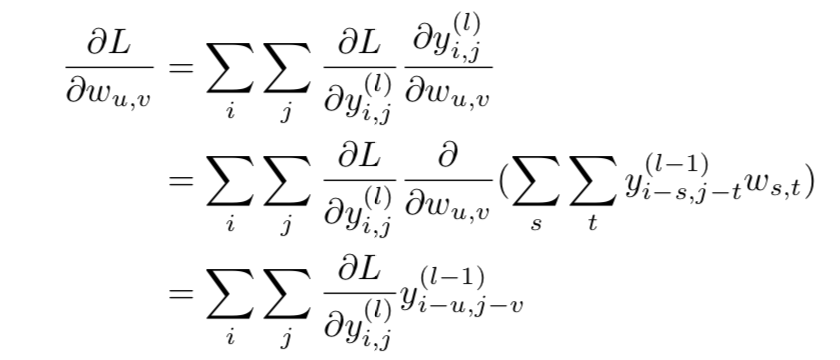
\includegraphics[scale=.3]{images/BackpropCNN.png}
    
    
    \textbf{Convolution stages:} the convolutional layer includes a convolution stage (affine transform), a detector stage (nonlinearity e.g. rectified linear) and a pooling stage (e.g. max pooling, average, soft-maximization). Only then do you move on to the next layer. \textbf{Convolutional Pyramid:} typical use of convoluton in vision: sequence of convolutions that reduce spatial dimensiosn (sub-sampling) and increase the number of channels.
    
    \textbf{1x1 'Convolution' as dimension reduction}: 
    % A convolutional layer is essentially a sum of the result of matrix multiplications for each of the previous layer's channels. The number of channels output by a set of filters is the number of filters. A 1x1 convolution therefore corresponds to a weighted sum for each pixel across all input channels, performed with a different set of weights for each 1x1 filter. Basically blends filters together. 
    For $m$ channels of a $1\times1\times k$ conv. $m\leq k:\vx^+_{ij}=\sigma(\vW\vx_{ij}),\>\vW\in\R^{m\times k}$ 
    
    \textbf{Computing the size of the output image after applying a kernel:} We apply $m$ $f$x$f$ filters to an $n \cross n \cross d$ image, padding $p$, stride $s$. For each dimension of the image: $L=\frac{n+2p-f}{s}+1$ Depth if going to be equal to the number m of filters.
    In general, setting zero padding to be $p=(f-1)/2$ when the stride is $s=1$ ensures that the input volume and output volume will have the same size spatially.
   \textbf{ With parameter sharing,} it introduces $f \cdot f \cdot d $ weights per filter, for a total of $(f\cdot f\cdot d)\cdot K$ weights and $K$ biases.
